\documentclass[11pt]{beamer} %Add 'handout' in the options for printing

\usepackage{beamercolorthemewolverine}
\usetheme{AnnArbor}

\usepackage[english]{babel}
\usepackage{amsmath,amssymb}
\usepackage{commath}
\usepackage{amssymb,amscd,amsfonts,amsbsy}
\usepackage{enumerate}
\usepackage{epsfig}
\usepackage{pgfpages}
\usepackage{graphics}
\usepackage{graphicx}
\usepackage{multicol}
\usepackage{layouts}
\usepackage[center]{caption}
\usepackage{natbib}
\usepackage{movie15}
\usepackage{etex}
%\usepackage{dsfont}
\usepackage{embedfile}
%\usepackage[natbib=true, bibstyle=authoryear, citestyle=authoryear-comp]{biblatex}
%\usepackage{apacite} 

\embedfile{Slides_Template.tex}

\setbeamertemplate{navigation symbols}{}%remove navigation symbols

\graphicspath{ {./figs/} }


% Figures within a column...
\makeatletter
\newenvironment{tablehere}
{\def\@captype{table}}
{}
\newenvironment{figurehere}
{\def\@captype{figure}}
{}
\makeatother

\newcommand{\beginbackup}{
   \newcounter{framenumbervorappendix}
   \setcounter{framenumbervorappendix}{\value{framenumber}}
}
\newcommand{\backupend}{
   \addtocounter{framenumbervorappendix}{-\value{framenumber}}
   \addtocounter{framenumber}{\value{framenumbervorappendix}} 
}

%---------------------------------------------------------------------------
\setbeamercolor{alerted text}{fg=red} 
\setbeamertemplate{frametitle}
{\vskip-18.5pt 
  \leavevmode
  \hbox{%
  \begin{beamercolorbox}[wd=\paperwidth,ht=1.35ex,dp=1.35ex]{frametitle}%
    \raggedright\hspace*{2em}\vspace{-7pt}\small{\insertframetitle}
  \end{beamercolorbox}
  }%
}
\def\newblock{\hskip .11em plus .33em minus .07em}

\setbeamercovered{dynamic}

\newcommand{\RR}{{\mathbb{R}}}
\newcommand{\NN}{{\mathbb{N}}}
\newcommand{\ZZ}{{\mathbb{Z}}}
\newcommand{\CC}{{\mathbb{C}}}
\newcommand{\eps}{\varepsilon}
\newcommand{\bp}{\noindent {\it Proof}.\,\,\,}
\newcommand{\ep}{\hfill$\Box$ \vskip 0.08in}
\newcommand{\dint}{\int\!\!\!\int}
\newcommand{\vs}{\vskip 0.5cm}
\newcommand{\po}{{\partial\Omega}}
\newcommand{\meanint}{{\int{\mkern-19mu}-}}
\def\ring{\mathaccent"0017 }


\title[Research Summary]{Presentation Title}
\author[Author Name] {}

\institute[UM]{}
\date[\today]{}

\begin{document}
\frame{ \vspace{-1cm}

\titlepage \vspace{-2.70cm}
\centering
\begin{columns}
\column{.25\textwidth}
\begin{figure} \centering 
\includegraphics[width=.75\columnwidth]{MichiganSeal} \end{figure}
\column{.5\textwidth} \begin{center}
\normalsize{Your name here} \vspace{4pt} \\ \footnotesize{Your lab here} \vspace{4pt}\\
\footnotesize{University of Michigan, Ann Arbor} \vspace{4pt} \\ \scriptsize{Department of Stuff Engineering} \vspace{4pt} \end{center}
\column{.25\textwidth}
\begin{figure} \centering 
\includegraphics[width=.75\columnwidth]{MElogo} \end{figure}
\end{columns}
\vspace{.45cm}
\begin{center}
\footnotesize {\today} \vspace{-.45cm}
\end{center}
\vspace{\fill}
}





\begin{frame}
\frametitle{Here's my first frame title}

\begin{center}
{\small Here are some pictures of bubbles}
\end{center}

\begin{figure}
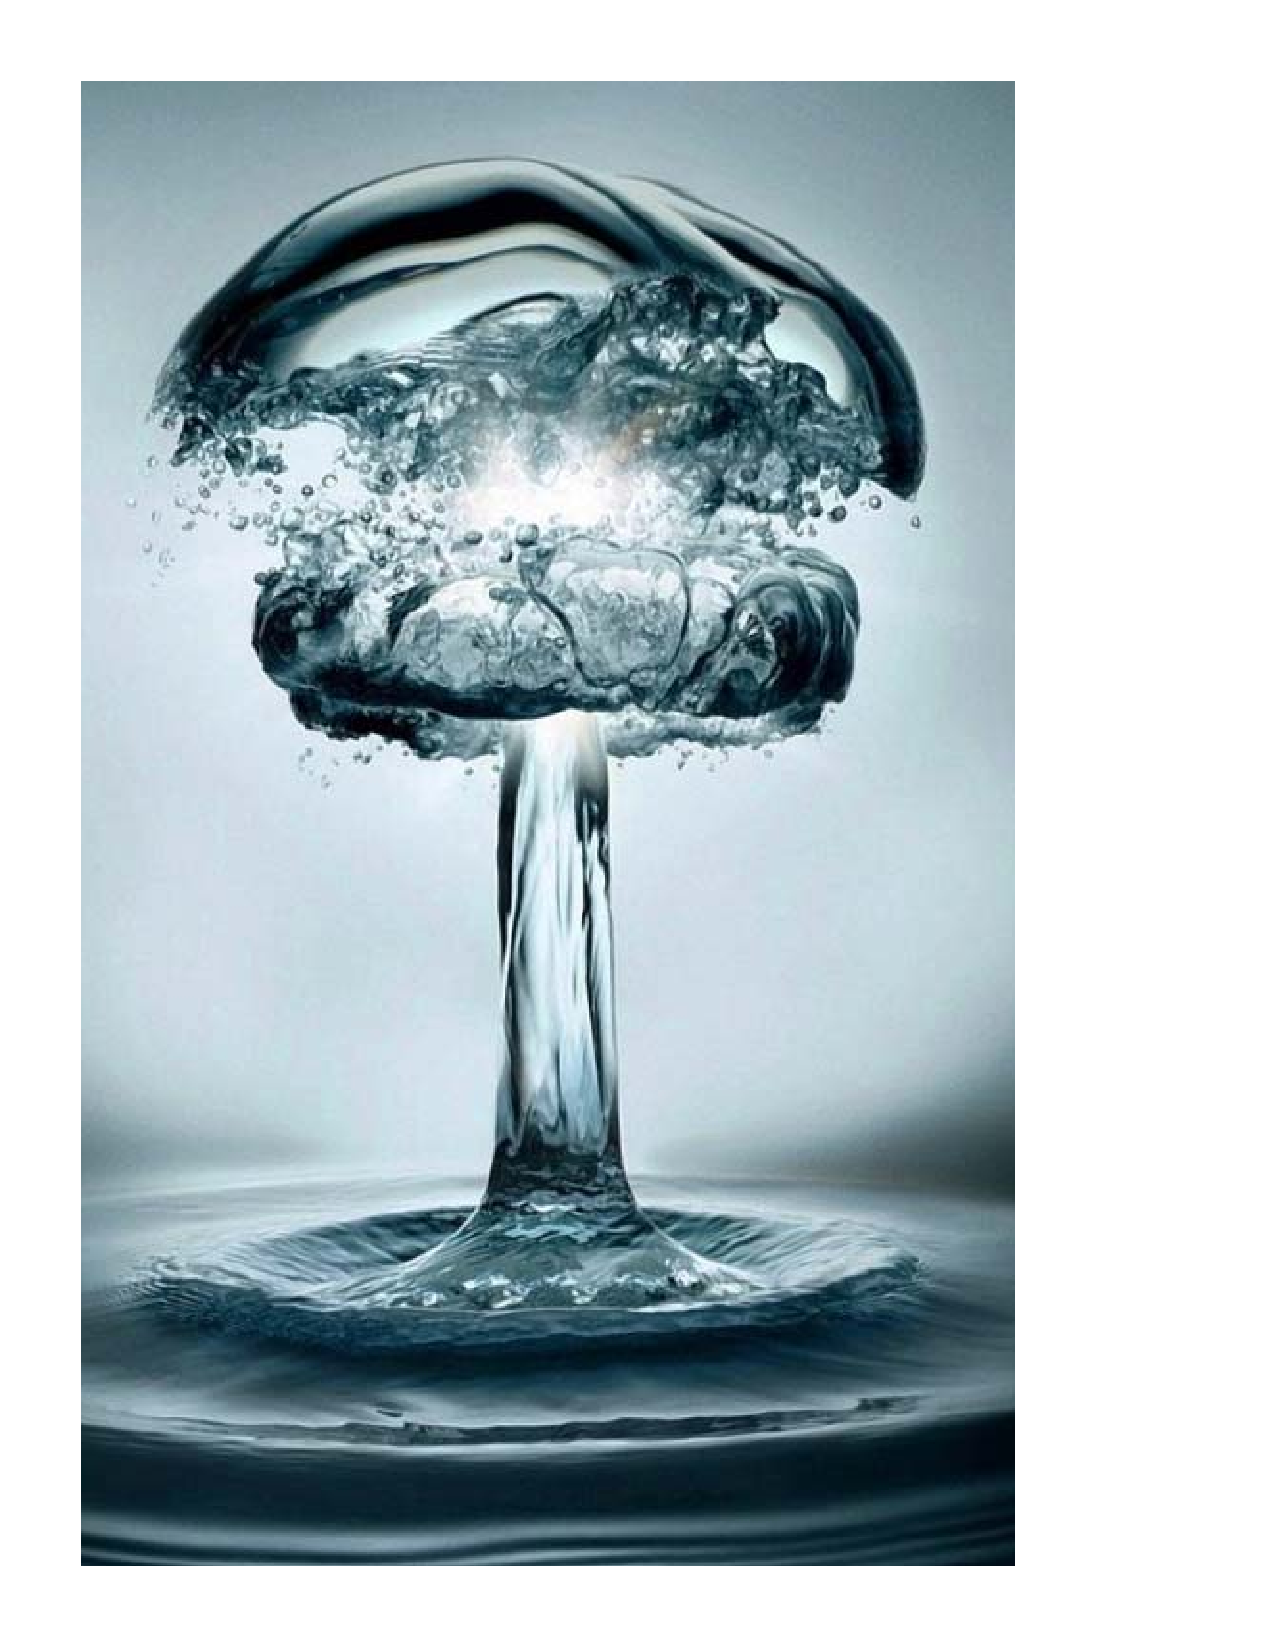
\includegraphics[width=.3\textwidth]{Undex} \hspace*{.2cm}
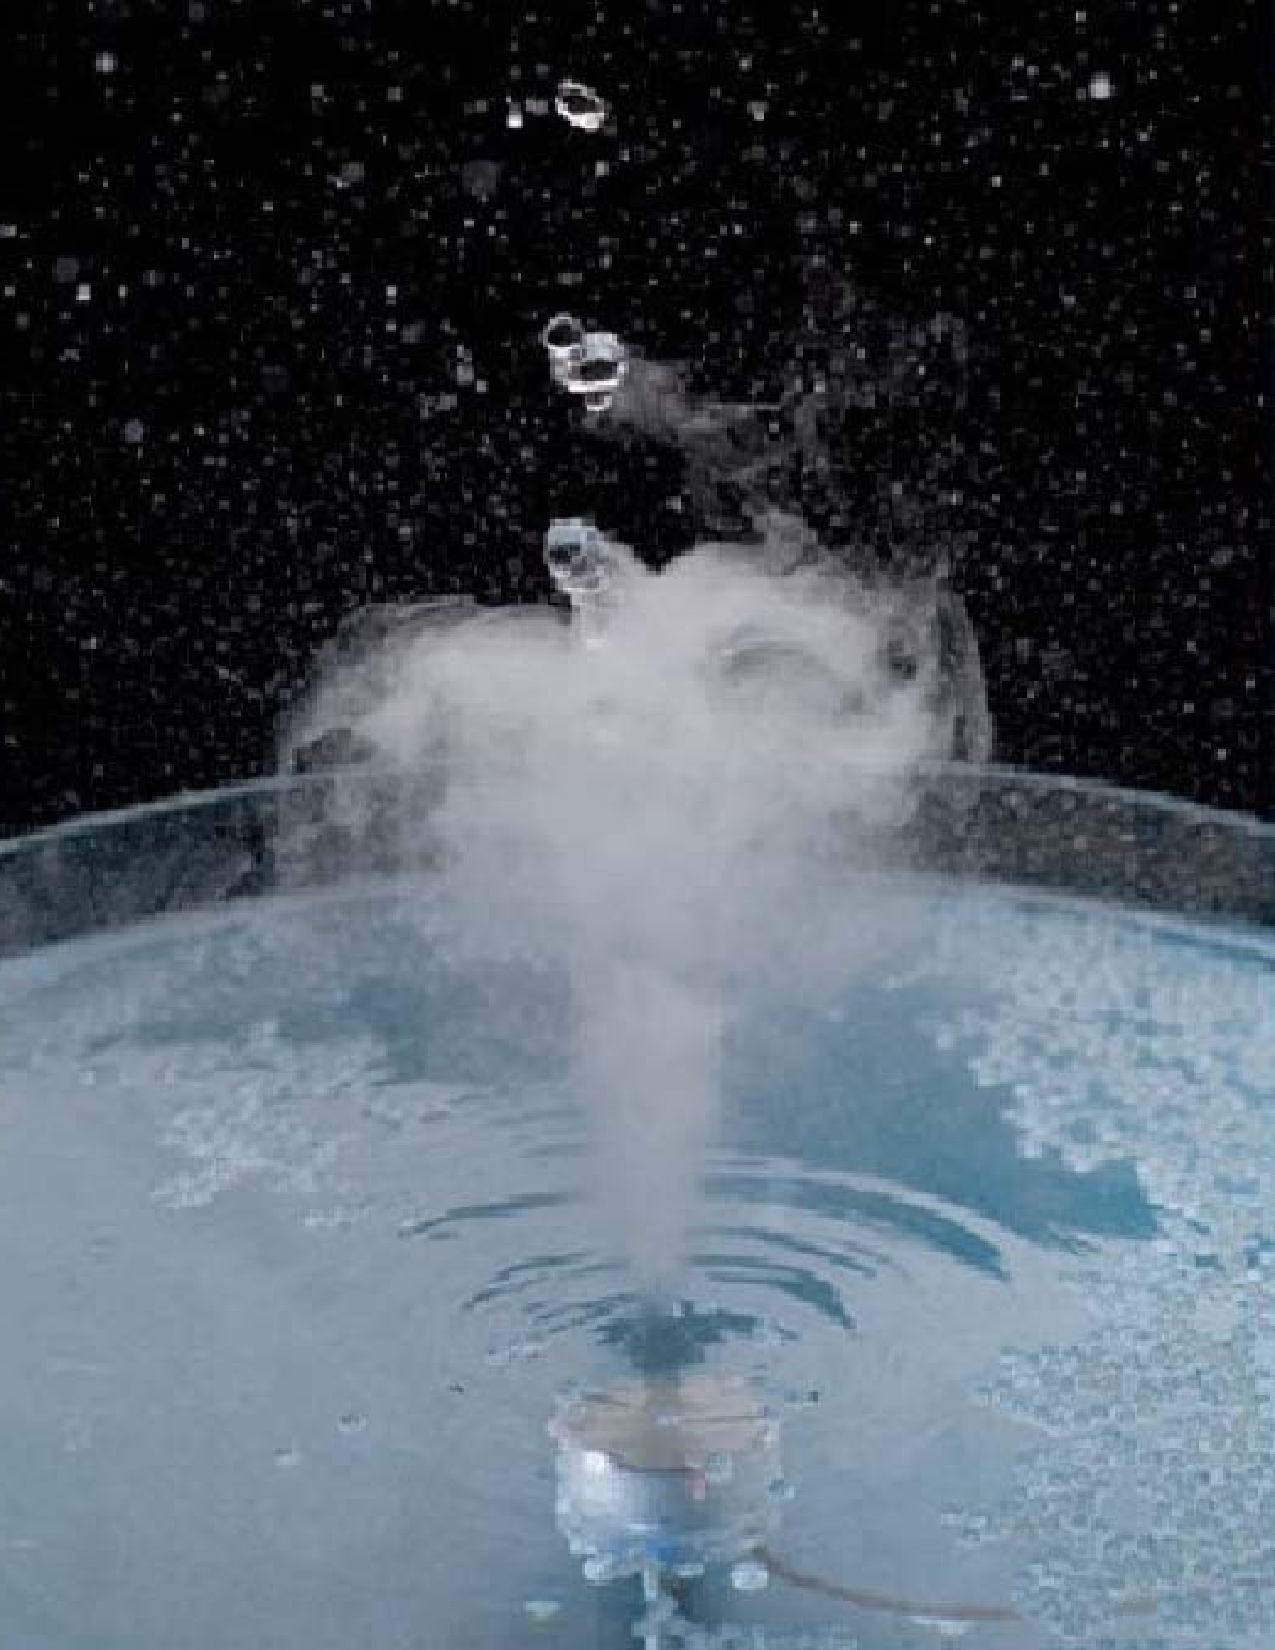
\includegraphics[width=.3\textwidth, height=.65\textheight]{Ultracav} \hspace*{.2cm}
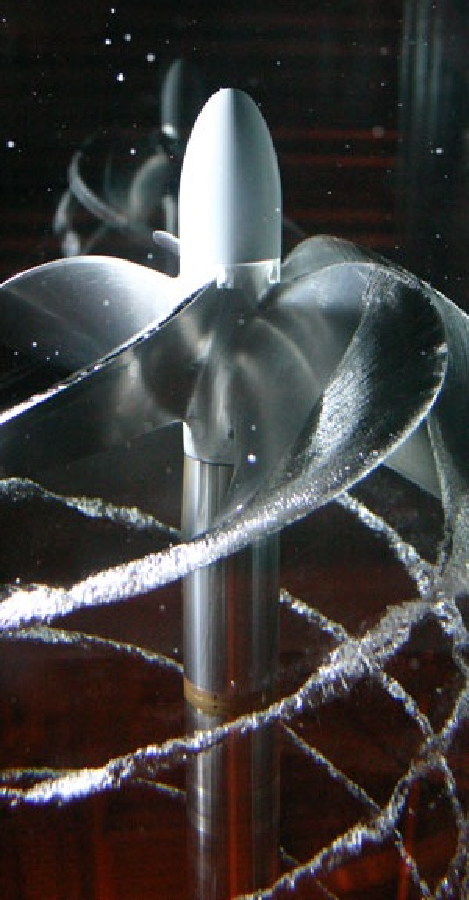
\includegraphics[width=.3\textwidth, height=.65\textheight]{propeller}\\ 
\hspace*{-.6cm}
\alert{Underwater Explosions \quad Ultrasound Probes \qquad Rotating Propellers}
\end{figure}
{\small I put some words here for filler when I'm giving a real presentation.  Some audiences like that, I'm not sure why.} 
\end{frame}

\begin{frame}
This slide can act as an example of sequentially changing pictures.
\begin{itemize}
\item Bullet points are nice.
\item You don't have to say much to take up space.
\item If you have dynamic slides like this, use the [handout] option in the document class at the top to condense animations for printing.
\end{itemize}
\vspace{-.5cm}
\begin{figure} 
\invisible<1>{\includegraphics<1>[width=.99\textwidth]{CavEvent1}}
\includegraphics<2>[width=\textwidth]{CavEvent1}
\includegraphics<3>[width=\textwidth]{CavEvent2}
\includegraphics<4>[width=\textwidth]{CavEvent3}
\includegraphics<5>[width=\textwidth]{CavEvent4}
\includegraphics<6>[width=\textwidth]{CavEvent5}
\only<7->{ 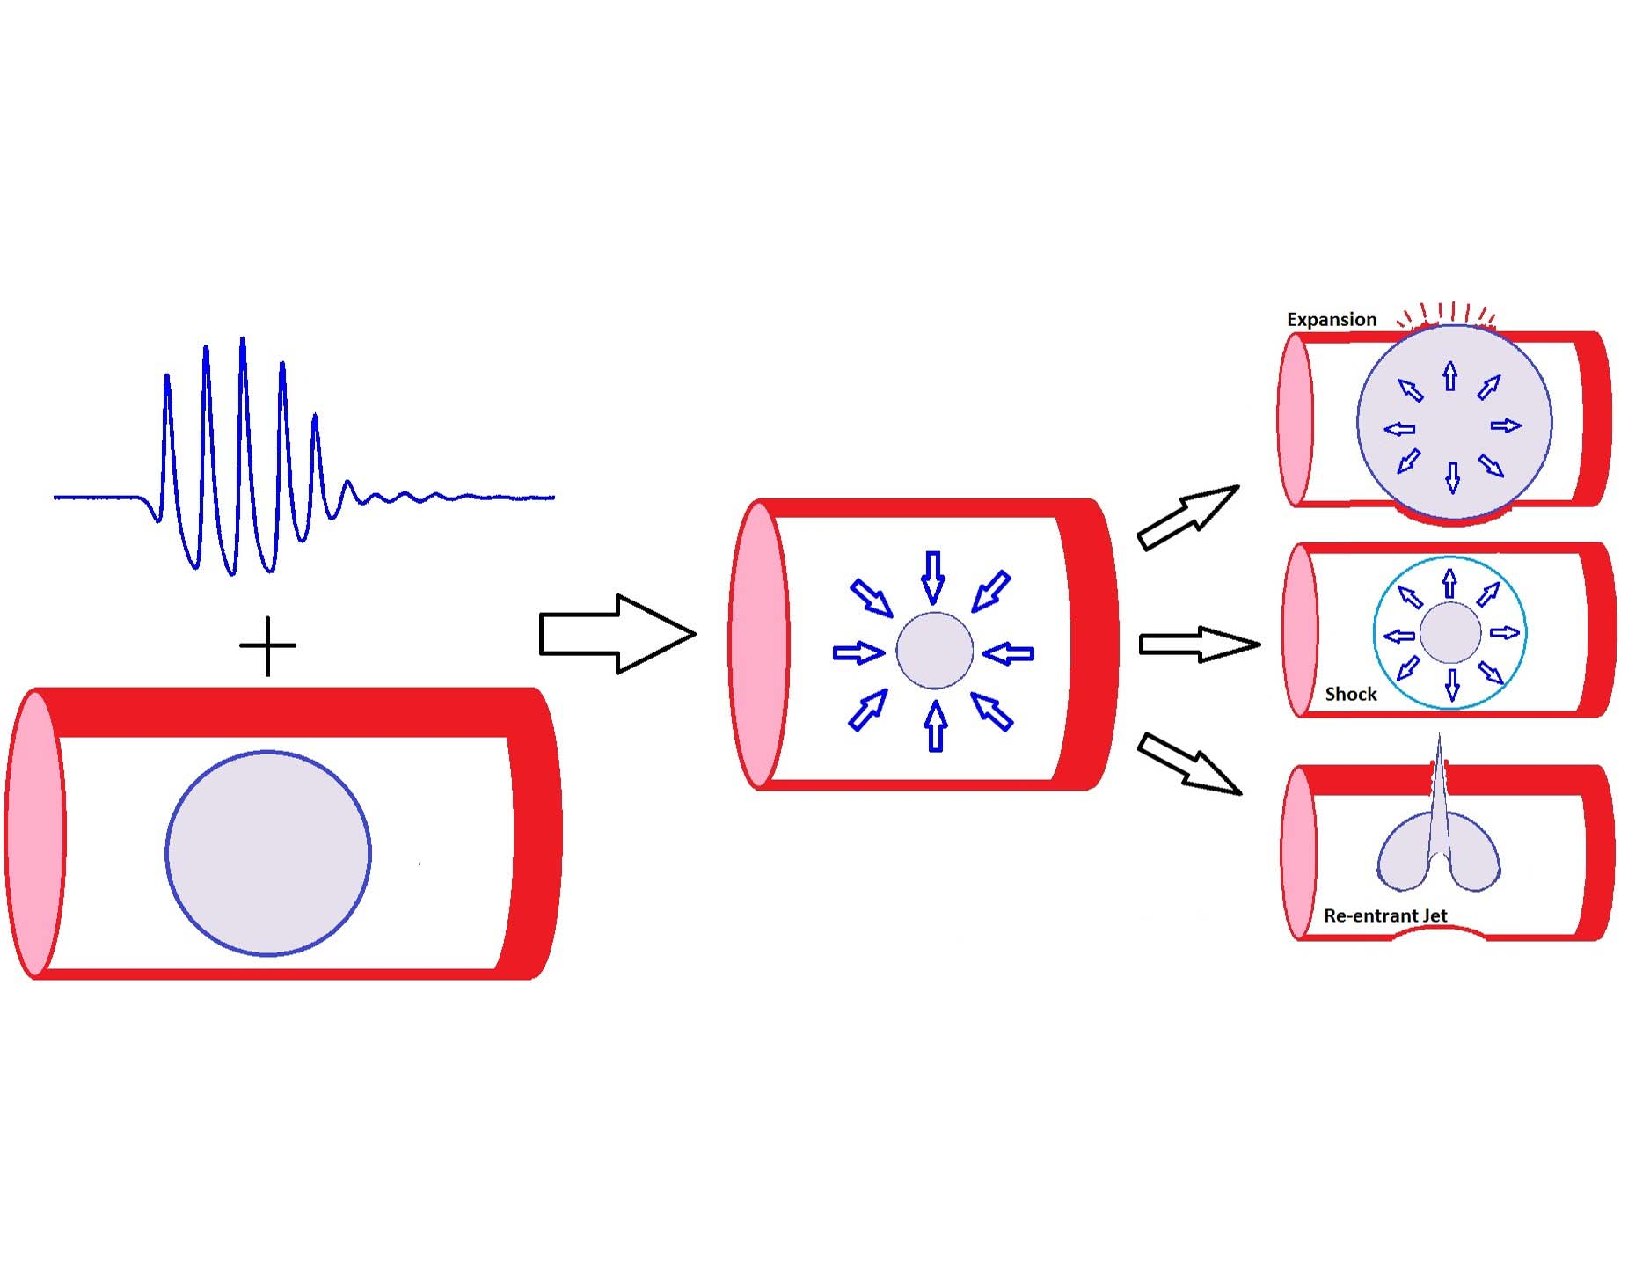
\includegraphics[width=.95\textwidth]{BleedMechs2}}
\end{figure} 
\end{frame}



\begin{frame}\frametitle{Normally I talk about my research here}
{\small
I kept this slide because it shows how to imbed a video into the slide.  I recommend mp4 because it works on most platforms.
\begin{minipage}{.58\textwidth}
\begin{itemize}
\item bullet 1
\item bullet 2 
\item etc...
\end{itemize}
\end{minipage}
}
\begin{minipage}{.4\textwidth}
%\begin{figure} \vspace*{-.15cm}
%\includemovie[poster,text={\small(Loading Video...)},rate=.5]{\textwidth}{.45\textwidth}{histotripsy.mp4}
%\end{figure}
\%\end{minipage}
\vspace*{0.5cm}
{\small 
\uncover<3>{
\\To organize this page, I used the minipage environment, it's handy for slides.
\begin{minipage}{.5\textwidth}
\begin{itemize}
\item Here, talk about the pictures and stuff
\item That pictures of a bloody kidney
\item You can put whatever picture you want there.
\end{itemize}
\vspace*{\fill}
\end{minipage}
\begin{minipage}{.45\textwidth}
\begin{figure}
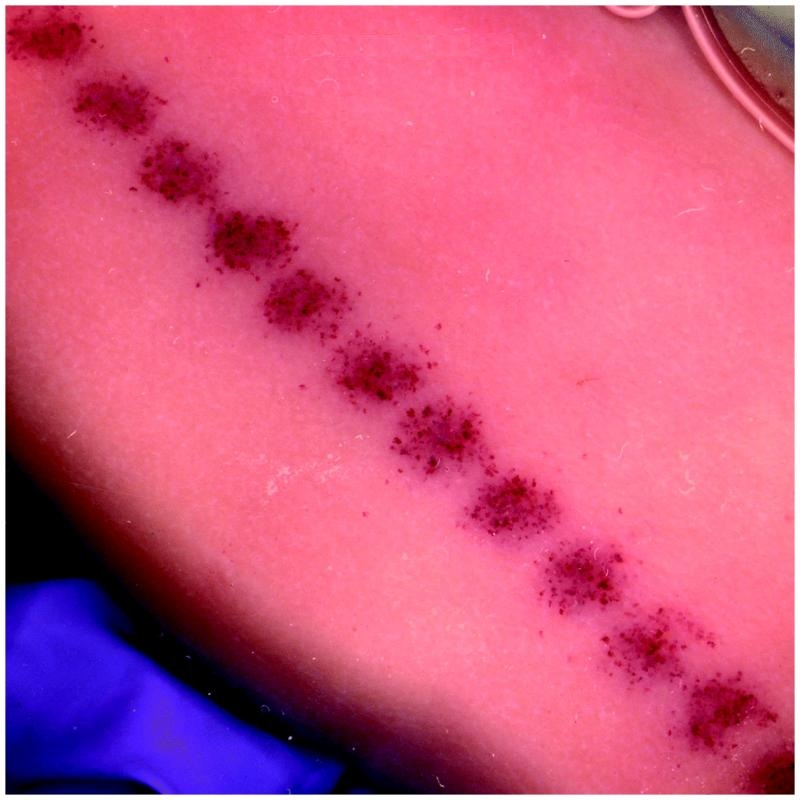
\includegraphics[width=\textwidth]{Kidney_Bleed}
\end{figure}
\end{minipage}
}}
\end{frame}


\section{Methods}
\subsection{Bubble Simulation}


\frame{
\vspace{.2cm}
\uncover<1->{\alert<1->{The Keller-Miksis Equation} \scriptsize{
\begin{align*}
	 \left(1-\frac{\dot{R}}{Ma}\right) R \ddot{R} + \frac{3}{2}\left(1-\frac{\dot{R}}{3 Ma}\right)\dot{R}^2 = \frac{R}{Ma}\left(\left(1+\frac{2}{We}\right) \frac{3\gamma}{R^{3\gamma+1}}\dot{R}+\frac{2 \dot{R}}{We R^2}  +  \dot{\tau}_{RR}  \right)
\end{align*}\vspace{-.4cm}
\begin{align*}
+ \left(1+\frac{\dot{R}}{Ma}\right)\left[\left(1+\frac{2}{We}\right)\frac{1}{R^{3\gamma}}-\frac{2}{We R}  + \tau_{RR}
	 -1-p_a(t)-\frac{R}{Ma} \dot{p}_a\right] \end{align*}}} \\ 
\pause 
\uncover<2->{ \normalsize{\alert<2->{Kelvin-Voigt} model for stress, $\tau_{rr}(R)$.  \normalsize
\vspace{-.85cm} 
\scriptsize{
\begin{columns} 
\column{.7\textwidth}
\begin{align*}
    \\ \tau_{rr} = -\frac{4}{3 Ca}\left(1-\frac{1}{R^{3}}\right)-\frac{4}{Re}\left( \frac{\dot{R}}{R}\right)
 \end{align*} 
 \column{.3\textwidth}
\begin{figure}
	\centering \vspace{.15cm} \invisible<1>{
\includegraphics<1->[width=\columnwidth]{Voigt}}
\end{figure}
 \end{columns}
 }}}

 \vspace{\fill} \pause
\vspace{-.3cm} \uncover<3->{
 \scriptsize \begin{center}
		\begin{tabular}{l l c l}
		  Parameter: & Dimensional & & Dimensionless \\ \hline
%		  Viscosity & $\mu=.015 \, \, \,  (Pa\cdot s)$ & $\mapsto$ & $Re=\rho R_0 c / \mu =2/3$ \\
		  Elasticity & $G=5,\alert{100},1000$ \,  $(kPa)$ & $\mapsto$ & $Ca=c^2 \rho / G=20,1,0.1$ 	\\
%		  Surface Tension & $s=.05\, \, \, (N/m)$ & $\mapsto$ & $We=\rho R_0 c^2 / s = 2$ \\
%		  Speed of Sound & $c_0=1570\, \, \, (m/s)$ & $\mapsto$ & $Ma=c_0/c=157$ \\  
%		  Relaxation Time & $t_c=0-1$  $(s)$ & $\mapsto$ &	$De=\lambda c / R_0=0-10^7$ \\
		  Initial Radius & $R(0)=0.1-2 \, \, \, (\mu m)$  & & \\
		  Adiabatic Index & $ $  $ $ & $ $ &	$\gamma=1.13,1.4$ \\

		\end{tabular}\\ \end{center}  \vspace{-.2cm}
		 \hspace{1.15cm}$R_0=1$ $\mu m$, $c = \sqrt{p_{atm}/\rho}$, $We=\rho R_0 c^2 / s$, $Re=\rho R_0 c / \mu$, $Ca= c^2\rho/G$, $Ma=c_0/c$}
		 \\ \hspace{1.15cm}\citep{HollandApfel90,YangChurch05}
}


\section{Conclusion}
\frame{
\frametitle{Summary and conclusions}
\begin{itemize}
\uncover<1->{\alert<1>{\item \LaTeX is sweet
\begin{itemize}
\item I've been recycling this presentation script since undergrad.
\end{itemize}} \vspace{.25cm}} %\pause
\uncover<2->{\alert<2>{\item If you want to learn more about LaTeX, there's tons of info online. \vspace{.25cm}}} 
\uncover<3->{\alert<3>{\item You can use this template as a starting point for building your own presentations. }}\vspace{.25cm} 
\vspace{\fill} \vspace{-.1cm}
\end{itemize}
}

\section{Citations}
\bibliography{mybib}
\bibliographystyle{authordate1}


%%%%%%%%%%%%%%%%%%%%%%%%%%%%%

\begin{frame} \vspace{\fill} \begin{center} \Huge 
Thanks a lot!\\ \vspace{\fill} Questions? 
\end{center} \vspace{\fill} \end{frame} 


\end{document}


%  Template Created by Brandon Patterson - awesome@umich.edu